%% ============================================================
%%  handout-aula01.tex — Resumo da Aula 1
%%  Aprendizagem por Reforço · UFU · Prof. Marcelo Keese Albertini
%%  Compilar com XeLaTeX (2x)
%% ============================================================
\documentclass[10pt, a4paper]{article}

\usepackage{fontspec}
\usepackage[margin=1.9cm, top=1.5cm, bottom=1.8cm]{geometry}
\usepackage{babel}
\babelprovide[import, main]{brazilian}
\usepackage{mathtools}
\usepackage{amssymb}
\usepackage[most]{tcolorbox}
\usepackage{tikz}
\usetikzlibrary{arrows.meta, positioning, calc}
\usepackage{multicol}
\usepackage{booktabs}
\usepackage{enumitem}
\usepackage{array}
\usepackage{fancyhdr}
\usepackage[hidelinks]{hyperref}

%% ---------------- cores (idênticas ao tema do curso) ----------
\definecolor{rlAzul}{HTML}{16324F}
\definecolor{rlAzulClaro}{HTML}{2E5F8A}
\definecolor{rlTeal}{HTML}{18808D}
\definecolor{rlLaranja}{HTML}{E8590C}
\definecolor{rlAmbar}{HTML}{F2A93B}
\definecolor{rlVermelho}{HTML}{C1121F}
\definecolor{rlVerde}{HTML}{2B9348}
\definecolor{rlCinza}{HTML}{5C677D}
\definecolor{rlFundo}{HTML}{FAFBFC}

%% ---------------- tipografia ----------------------------------
\IfFontExistsTF{Fira Sans}{%
  \setsansfont{Fira Sans}[
    ItalicFont = Fira Sans Italic,
    BoldFont = Fira Sans SemiBold,
    BoldItalicFont = Fira Sans SemiBold Italic]
}{\setsansfont{TeX Gyre Heros}}
\IfFontExistsTF{Fira Mono}{\setmonofont{Fira Mono}[Scale=0.88]}%
  {\setmonofont{Latin Modern Mono}[Scale=0.9]}
\renewcommand{\familydefault}{\sfdefault}

\setlength{\parindent}{0pt}
\setlength{\parskip}{0.45em}
\linespread{1.03}

%% ---------------- cabeçalho / rodapé --------------------------
\pagestyle{fancy}
\fancyhf{}
\renewcommand{\headrulewidth}{0pt}
\renewcommand{\footrulewidth}{0.4pt}
\renewcommand{\footrule}{{\color{rlAzul!20}%
  \vskip-\footruleskip\vskip-0.4pt\hrule width\headwidth height0.4pt\vskip\footruleskip}}
\fancyfoot[L]{\footnotesize\color{rlCinza}Aprendizagem por Reforço \textbullet\ Aula 1}
\fancyfoot[R]{\footnotesize\color{rlCinza}\thepage\,/\,\pageref{ultimapagina}}

%% ---------------- títulos de seção ----------------------------
\newcounter{secao}
\newcommand{\secao}[1]{%
  \stepcounter{secao}%
  \vspace{0.7em}%
  \noindent{\color{rlLaranja}\rule{1.6em}{2pt}}\hspace{0.5em}%
  {\color{rlCinza}\footnotesize\bfseries\thesecao}\hspace{0.35em}%
  {\color{rlAzul}\large\bfseries #1}%
  \par\vspace{-0.15em}%
  {\color{rlAzul!22}\rule{\linewidth}{0.6pt}}%
  \par\vspace{0.25em}}

\newcommand{\subt}[1]{\vspace{0.35em}\noindent{\color{rlAzulClaro}\bfseries #1}\par
  \vspace{-0.25em}}

%% ---------------- caixas --------------------------------------
\tcbset{hcaixa/.style={
  enhanced, boxrule=0pt, frame hidden, arc=1.2mm,
  left=2.2mm, right=2.2mm, top=1.2mm, bottom=1.4mm, boxsep=0.7mm,
  before skip=0.7em, after skip=0.7em,
  borderline west={2.2pt}{0pt}{#1},
  colback=rlFundo, fonttitle=\bfseries\small, coltitle=#1,
  attach title to upper={\par\vspace{0.3ex}},
}}
\newtcolorbox{defbox}[2][]{hcaixa=rlTeal, title={Definição — #2}, #1}
\newtcolorbox{ideiabox}[1][]{hcaixa=rlAmbar, title={Intuição},
  colback=rlAmbar!9, coltitle=rlLaranja, #1}
\newtcolorbox{alertabox}[1][]{hcaixa=rlVermelho, title={Atenção},
  colback=rlVermelho!5, #1}
\newtcolorbox{algbox}[2][]{hcaixa=rlAzul, title={Algoritmo — #2},
  colback=rlAzul!5, #1}
\newtcolorbox{chave}[1][]{hcaixa=rlVerde, title={Ideia central},
  colback=rlVerde!6, #1}

% caixinha compacta para os "quatro ingredientes"
\newtcolorbox{ingr}[1]{enhanced, arc=1.2mm, boxrule=0.7pt,
  colframe=rlAzul!18, colback=white,
  left=2.2mm, right=2.2mm, top=1.4mm, bottom=1.6mm, boxsep=0.6mm,
  fonttitle=\bfseries\small, coltitle=rlAzul, title={#1},
  attach title to upper={\par\vspace{0.3ex}}, fontupper=\footnotesize}

%% ---------------- macros matemáticas (as do curso) ------------
\newcommand{\E}{\mathbb{E}}
\newcommand{\Prob}{\mathbb{P}}
\newcommand{\R}{\mathbb{R}}
\newcommand{\gS}{\mathcal{S}}
\newcommand{\gA}{\mathcal{A}}
\newcommand{\pol}{\pi}
\newcommand{\tran}[2]{P(#1\mid #2)}
\newcommand{\rec}{R}
\DeclareMathOperator*{\argmax}{arg\,max}
\DeclarePairedDelimiter{\abs}{\lvert}{\rvert}
\DeclarePairedDelimiter{\norm}{\lVert}{\rVert}
\newcommand{\norminf}[1]{\norm{#1}_{\infty}}
\newcommand{\termo}[2]{\underbrace{#1}_{\text{\scriptsize\color{rlCinza}#2}}}

\hyphenation{apren-di-za-gem re-com-pen-sa se-quen-cial de-ter-mi-nís-ti-ca}

%% ============================================================
\begin{document}

%% ---------------- faixa de título -----------------------------
\begin{tikzpicture}[remember picture, overlay]
  \fill[rlAzul] ([yshift=0cm]current page.north west)
    rectangle ([yshift=-3.15cm]current page.north east);
  \node[anchor=north west, text width=0.70\paperwidth, inner sep=0pt]
    at ([xshift=1.9cm, yshift=-0.78cm]current page.north west) {%
      {\color{rlAmbar}\footnotesize\bfseries
       UNIVERSIDADE FEDERAL DE UBERLÂNDIA \ \textbullet\ \ APRENDIZAGEM POR REFORÇO}\\[0.4em]
      {\color{white}\Large\bfseries Aula 1 — Introdução à aprendizagem por reforço}\\[0.35em]
      {\color{white!72!rlAzul}\small Resumo de estudo \ \textbullet\ \
       decisão sequencial, processos de Markov e a equação de Bellman}};
  \node[anchor=north east, text width=5.2cm, align=right, inner sep=0pt]
    at ([xshift=-1.9cm, yshift=-0.8cm]current page.north east) {%
      {\color{white!70!rlAzul}\scriptsize Prof.\ Marcelo Keese Albertini\\[0.15em]
       adaptado de CS234, Stanford}};
\end{tikzpicture}
\vspace*{1.55cm}

\begin{chave}
Aprendizagem por reforço é aprender, a partir de \textbf{experiência}, a tomar
\textbf{boas decisões} sob \textbf{incerteza}. O que a distingue dos demais
paradigmas: os dados que o agente verá amanhã dependem das decisões que ele
tomar hoje.
\end{chave}

%% ============================================================
\secao{Os quatro ingredientes}

\begin{multicols}{2}
\begin{ingr}{1. Otimização}
Buscamos a \emph{melhor} maneira de decidir, com uma noção explícita de
utilidade. Não basta prever bem — é preciso agir bem.
\end{ingr}

\begin{ingr}{2. Consequências adiadas}
A decisão de agora afeta resultados distantes. Cria dois problemas: pesar
futuro no \emph{planejamento} e a \emph{atribuição de crédito temporal} no
aprendizado.
\end{ingr}

\columnbreak

\begin{ingr}{3. Exploração}
O agente só observa a recompensa da ação que tomou. O resultado das
alternativas é um contrafactual que nunca se observa.
\end{ingr}

\begin{ingr}{4. Generalização}
A política precisa agir bem em estados nunca vistos — daí o uso de
aproximadores de função (redes neurais).
\end{ingr}
\end{multicols}

\vspace{-0.3em}
{\footnotesize\color{rlCinza}
Aprendizado supervisionado tem apenas o item 4; otimização clássica, apenas o
item 1; \emph{bandits} têm 1, 3 e 4. RL é o problema completo.}

%% ============================================================
\secao{Do laço agente--mundo ao estado de Markov}

A cada passo $t$: o agente executa $a_t$; o mundo se atualiza e emite
observação $o_t$ e recompensa $r_t$; o agente recebe ambas e decide $a_{t+1}$.

\begin{defbox}{história e estado}
\textbf{História:} $h_t = (a_1, o_1, r_1, \ldots, a_t, o_t, r_t)$ — tudo que o
agente fez e percebeu.\\
\textbf{Estado:} $s_t = f(h_t)$ — o resumo da história que assumimos suficiente
para determinar o que vem a seguir.
\end{defbox}

\begin{defbox}{estado de Markov}
$s_t$ é de Markov se, e somente se,
$\;\Prob(s_{t+1} \mid s_t, a_t) = \Prob(s_{t+1} \mid h_t, a_t)$,
isto é, $s_t$ é uma \emph{estatística suficiente} da história.
\end{defbox}

\begin{ideiabox}
``O futuro é independente do passado, dado o presente.'' Markov sempre pode ser
satisfeito trivialmente tomando $s_t = h_t$ — mas isso é inútil, pois o estado
explode. A arte está em achar o \emph{menor} resumo que ainda é (quase) Markov.
A escolha da representação de estado afeta diretamente o custo computacional, a
quantidade de dados necessária e o desempenho final.
\end{ideiabox}

\subt{Três eixos para classificar um problema}
\begin{itemize}[leftmargin=1.2em, itemsep=0.1ex, topsep=0.2ex]
  \item O estado é totalmente observável? Se não, é um \textbf{POMDP}.
  \item A dinâmica é determinística ou estocástica?
  \item As ações afetam apenas a recompensa imediata (\textbf{bandits}) ou
        também o próximo estado (problema sequencial completo)?
\end{itemize}

%% ============================================================
\secao{Cadeias de Markov e processos de recompensa}

\begin{defbox}{processo de Markov (cadeia)}
Par $(\gS, P)$: um conjunto finito de estados e um modelo de transição
$p(s_{t+1}=s' \mid s_t = s)$. \emph{Sem ações, sem recompensas.} Com $N$
estados, $P$ é uma matriz $N\times N$ cujas linhas somam 1.
\end{defbox}

\begin{defbox}{processo de recompensa de Markov (MRP)}
Quádrupla $(\gS, P, \rec, \gamma)$: acrescenta a função recompensa
$\rec(s) = \E[r_t \mid s_t = s]$ e o fator de desconto $\gamma \in [0,1]$.
\emph{Ainda sem ações.}
\end{defbox}

\subt{Horizonte, retorno e valor}
\vspace{-0.4em}
\begin{align*}
  G_t &= r_t + \gamma r_{t+1} + \gamma^2 r_{t+2} + \cdots
         + \gamma^{H-1} r_{t+H-1}
         &&\text{\footnotesize retorno (variável aleatória)}\\[0.15em]
  V(s) &= \E[\,G_t \mid s_t = s\,]
         &&\text{\footnotesize função valor (número por estado)}
\end{align*}
\vspace{-0.9em}

\begin{ideiabox}
O \emph{retorno} é o que aconteceu numa trajetória; o \emph{valor} é o que
esperamos em média. A função valor comprime toda a aleatoriedade futura em um
único número por estado — é o objeto que calculamos, estimamos e otimizamos no
curso inteiro.
\end{ideiabox}

\subt{Por que descontar}
$\gamma$ evita retornos infinitos quando $H=\infty$ e reflete a preferência
observada por recompensa imediata.
$\gamma = 0$: agente míope, $V(s)=\rec(s)$.
$\gamma = 1$: futuro vale tanto quanto o presente — seguro apenas se
$H < \infty$.

%% ============================================================
\secao{A equação de Bellman}

A propriedade de Markov dá estrutura recursiva ao problema:
\vspace{-0.3em}
\[
  V(s) \;=\; \termo{\rec(s)}{recompensa imediata}
    \;+\; \termo{\gamma \sum_{s' \in \gS} \tran{s'}{s}\, V(s')}%
                {soma descontada das recompensas futuras}
\]

Em forma vetorial, $V = \rec + \gamma P V$, de onde saem os dois métodos de
solução:

\subt{a) Solução analítica}
\vspace{-0.7em}
\[
  (I - \gamma P)\,V = \rec
  \quad\Longrightarrow\quad
  V = (I - \gamma P)^{-1}\rec
\]
\vspace{-0.9em}

Para $\gamma < 1$ a matriz $(I-\gamma P)$ é invertível e a solução é única.
Custo: $O(N^3)$.

\subt{b) Solução iterativa (programação dinâmica)}
\vspace{-0.4em}
\begin{algbox}{avaliação iterativa do valor de um MRP}
Inicialize $V_0(s) = 0$ para todo $s$. Para $k = 1, 2, \ldots$ até a
convergência, e para todo $s \in \gS$:
\[
  V_k(s) \;=\; \rec(s) + \gamma \sum_{s' \in \gS} \tran{s'}{s}\, V_{k-1}(s')
\]
Custo: $O(\abs{\gS}^2)$ \emph{por iteração}.
\end{algbox}

\vspace{-0.4em}
\begin{ideiabox}
A iteração converge porque o operador de Bellman é uma \emph{contração}:
o erro cai geometricamente, $\norminf{V_k - V} \le \gamma^k \norminf{V_0 - V}$.
A prova vem na Aula 2 — por ora, observe o efeito na tabela da seção seguinte.
\end{ideiabox}

%% ============================================================
\secao{Exemplo trabalhado: \emph{Mars Rover}}

Sete posições; a cada passo o rover vai para cada lado com probabilidade
$0{,}4$ e permanece com o restante; as bordas absorvem o excedente.
Recompensa $+1$ em $s_1$, $+10$ em $s_7$, $0$ nos demais. Tome
$\gamma = 0{,}9$.

\vspace{0.2em}
\begin{center}
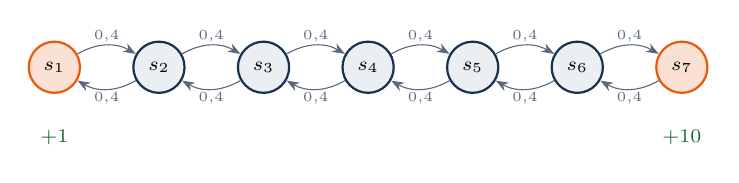
\begin{tikzpicture}[node distance=6.5mm, scale=1, transform shape]
  \tikzset{
    est/.style={circle, draw=rlAzul, thick, fill=rlAzul!8,
                minimum size=6.5mm, inner sep=0pt, font=\scriptsize},
    estd/.style={est, fill=rlLaranja!18, draw=rlLaranja}}
  \node[estd] (s1) {$s_1$};
  \foreach \i/\p in {2/1,3/2,4/3,5/4,6/5} \node[est, right=of s\p] (s\i) {$s_\i$};
  \node[estd, right=of s6] (s7) {$s_7$};
  \foreach \i/\j in {1/2,2/3,3/4,4/5,5/6,6/7}{
    \draw[-{Stealth[length=1.6mm]}, rlCinza] (s\i) to[bend left=30]
      node[font=\tiny, above, inner sep=1pt, text=rlCinza] {$0{,}4$} (s\j);
    \draw[-{Stealth[length=1.6mm]}, rlCinza] (s\j) to[bend left=30]
      node[font=\tiny, below, inner sep=1pt, text=rlCinza] {$0{,}4$} (s\i);}
  \node[font=\scriptsize, text=rlVerde!70!black, below=3.4mm of s1] {$+1$};
  \node[font=\scriptsize, text=rlVerde!70!black, below=3.4mm of s7] {$+10$};
\end{tikzpicture}
\end{center}

\vspace{-0.2em}
\begin{center}
\footnotesize
\setlength{\tabcolsep}{5.2pt}
\renewcommand{\arraystretch}{1.12}
\begin{tabular}{@{}l rrrrrrr @{\hspace{1.4em}} r@{}}
  \toprule
  $k$ & $s_1$ & $s_2$ & $s_3$ & $s_4$ & $s_5$ & $s_6$ & $s_7$
      & $\norminf{V_k - V}$ \\
  \midrule
  0 & 0{,}00 & 0{,}00 & 0{,}00 & 0{,}00 & 0{,}00 & 0{,}00 & 0{,}00 & 40{,}97 \\
  1 & 1{,}00 & 0{,}00 & 0{,}00 & 0{,}00 & 0{,}00 & 0{,}00 & 10{,}00 & 30{,}97 \\
  2 & 1{,}54 & 0{,}36 & 0{,}00 & 0{,}00 & 0{,}00 & 3{,}60 & 15{,}40 & 25{,}57 \\
  3 & 1{,}96 & 0{,}62 & 0{,}13 & 0{,}00 & 1{,}30 & 6{,}19 & 19{,}61 & 21{,}36 \\
  4 & 2{,}28 & 0{,}86 & 0{,}25 & 0{,}51 & 2{,}46 & 8{,}64 & 22{,}82 & 18{,}15 \\
  5 & 2{,}54 & 1{,}07 & 0{,}54 & 1{,}07 & 3{,}74 & 10{,}66 & 25{,}43 & 15{,}54 \\
  \midrule
  \multicolumn{1}{@{}l}{$V$ (exato)}
    & \textbf{6{,}91} & \textbf{6{,}05} & \textbf{6{,}87} & \textbf{9{,}61}
    & \textbf{15{,}01} & \textbf{24{,}58} & \textbf{40{,}97} & --- \\
  \bottomrule
\end{tabular}
\end{center}

\vspace{-0.2em}
\textbf{O que ler nesta tabela.}
\begin{itemize}[leftmargin=1.2em, itemsep=0.15ex, topsep=0.2ex]
  \item O valor \emph{se espalha} a partir das fontes de recompensa: em $k=1$
        só $s_1$ e $s_7$ têm valor; a informação leva uma iteração para andar
        um estado. Em $k=3$ ela ainda não chegou a $s_4$.
  \item Na solução exata, $V(s_2) < V(s_1)$ e $V(s_3) < V(s_1)$, mas
        $V(s_4) > V(s_1)$: perto da borda esquerda vale a pena o $+1$ fácil;
        do meio para a direita, o $+10$ domina apesar de mais distante.
  \item A razão entre erros sucessivos ($0{,}76;\ 0{,}83;\ 0{,}84;\ 0{,}85;
        \ldots$) sobe em direção a $\gamma = 0{,}9$ — exatamente a taxa de
        contração prevista.
\end{itemize}

%% ============================================================
\secao{Armadilhas comuns}

\begin{alertabox}
\begin{itemize}[leftmargin=1.1em, itemsep=0.25ex, topsep=0.2ex, parsep=0pt]
  \item \textbf{Confundir retorno com valor.} $G_t$ é aleatório e vale para
        \emph{uma} trajetória; $V(s)$ é a esperança sobre todas elas.
  \item \textbf{Achar que política determinística implica trajetória
        determinística.} A política pode ser determinística e o ambiente
        estocástico: ações fixas, resultados variados.
  \item \textbf{Usar $\gamma = 1$ com horizonte infinito.} A soma pode
        divergir e $(I - \gamma P)$ deixa de ser invertível.
  \item \textbf{Tratar o modelo do agente como verdade.} No exemplo do CS234,
        o modelo de recompensa do rover prevê $\hat r = 0$ em todo estado — e
        está errado. Agir bem apesar disso é boa parte do curso.
  \item \textbf{Projetar recompensa ingenuamente.} O agente otimiza o que foi
        escrito, não o que se quis dizer: um tutor recompensado por acertos
        aprende a propor só exercícios fáceis.
\end{itemize}
\end{alertabox}

%% ============================================================
\secao{Notação e vocabulário}

\begin{multicols}{2}
{\footnotesize
\begin{tabular}{@{}l l@{}}
  \toprule
  \textbf{Símbolo} & \textbf{Significado} \\
  \midrule
  $\gS$, $\gA$ & espaços de estados e ações \\
  $s_t$, $a_t$, $r_t$ & estado, ação, recompensa em $t$ \\
  $h_t$ & história até $t$ \\
  $P(s'\mid s)$ & modelo de transição \\
  $\rec(s)$ & recompensa esperada em $s$ \\
  $\gamma$ & fator de desconto \\
  $H$ & horizonte \\
  $G_t$ & retorno a partir de $t$ \\
  $V(s)$ & função valor de estado \\
  $\pol$ & política \\
  $\norminf{\cdot}$ & norma do supremo \\
  \bottomrule
\end{tabular}}

\columnbreak

{\footnotesize
\begin{tabular}{@{}l l@{}}
  \toprule
  \textbf{Inglês} & \textbf{Português} \\
  \midrule
  reinforcement learning & aprendizagem por reforço \\
  state / action / reward & estado / ação / recompensa \\
  policy & política \\
  value function & função valor \\
  return & retorno \\
  horizon & horizonte \\
  discount factor & fator de desconto \\
  transition model & modelo de transição \\
  policy evaluation & avaliação de política \\
  contraction operator & operador de contração \\
  \emph{backup} & mantido em inglês \\
  \bottomrule
\end{tabular}}
\end{multicols}

%% ============================================================
\secao{Exercícios}

\begin{enumerate}[leftmargin=1.4em, itemsep=0.4ex, topsep=0.2ex]
  \item \textbf{Caso míope.} Mostre que, com $\gamma = 0$, a iteração converge
        em um único passo e $V(s) = \rec(s)$ para todo $s$.
  \item \textbf{Propagação.} Sem calcular tudo, argumente quantas iterações são
        necessárias para que $V_k(s_4) > 0$ no exemplo acima. Generalize: qual
        a relação entre o número de iterações e a distância até a fonte de
        recompensa mais próxima?
  \item \textbf{Onde fica o mínimo.} Com $\gamma = 0{,}5$, a solução exata é
        $V = (1{,}53;\ 0{,}37;\ 0{,}13;\ 0{,}22;\ 0{,}85;\ 3{,}59;\ 15{,}31)$.
        Em qual estado está o \emph{menor} valor nesse caso? E na tabela de
        $\gamma = 0{,}9$? Explique por que o mínimo se desloca.
  \item \textbf{Custos.} Para que valores de $N$ e de número de iterações $K$ a
        solução iterativa é mais barata que a analítica? Escreva a condição em
        função de $N$ e $K$.
  \item \textbf{Modelagem.} Modele como processo de decisão: um sistema de
        recomendação de vídeos que recebe $+1$ por clique. Defina estado, ação e
        recompensa; depois aponte qual comportamento indesejado essa recompensa
        pode induzir e proponha uma alternativa.
  \item \textbf{Markov ou não.} Para cada caso, diga se a representação é de
        Markov e justifique: (a) tabuleiro de xadrez atual mais jogador da vez;
        (b) um único quadro de um jogo de Atari com objetos em movimento;
        (c) os quatro últimos quadros do mesmo jogo.
\end{enumerate}

%% ============================================================
\secao{Respostas resumidas}

{\footnotesize
\begin{enumerate}[leftmargin=1.4em, itemsep=0.35ex, topsep=0.2ex]
  \item Com $\gamma = 0$ o termo futuro desaparece:
        $V_1(s) = \rec(s) + 0 = \rec(s)$, e $V_2 = V_1$. O ponto fixo é
        atingido na primeira iteração — o agente é míope por construção.
  \item $V_k(s) > 0$ apenas quando existe caminho de comprimento $\le k-1$ de
        $s$ até algum estado com recompensa. Como $s_4$ dista 3 passos tanto de
        $s_1$ quanto de $s_7$, é preciso $k \ge 4$ — e a tabela confirma:
        $V_4(s_4) = 0{,}51$ é o primeiro valor não nulo. Em geral, o valor se
        propaga um estado por iteração.
  \item Com $\gamma = 0{,}5$ o mínimo está em $s_3$; com $\gamma = 0{,}9$, em
        $s_2$. Desconto forte encolhe o alcance do $+10$, então o pior lugar é
        o mais distante do $+1$ que ainda não sente a borda direita. Com
        $\gamma = 0{,}9$ o $+10$ irradia por toda a cadeia e empurra o ponto de
        equilíbrio para a esquerda.
  \item Iterativa: $K \cdot O(N^2)$; analítica: $O(N^3)$. A iterativa é mais
        barata quando $K < N$. O detalhe importante: $K$ depende da precisão
        desejada e de $\gamma$
        ($K \approx \log \varepsilon / \log \gamma$), \emph{não} de $N$ —
        logo, para $N$ grande a iterativa praticamente sempre vence.
  \item Estado: histórico e perfil do usuário; ação: vídeo recomendado;
        recompensa: $+1$ por clique. O comportamento induzido é
        \emph{clickbait} — títulos sensacionalistas maximizam cliques sem
        entregar valor, e o sistema pode estreitar o interesse do usuário.
        Alternativas: tempo assistido em proporção à duração, avaliação
        explícita, ou retenção medida em janelas longas.
  \item (a) Sim, desde que o estado inclua também direitos de roque,
        possibilidade de \emph{en passant} e contadores de repetição — só o
        arranjo das peças não basta. (b) Não: um único quadro não informa
        velocidade nem direção dos objetos. (c) Aproximadamente sim — empilhar
        quatro quadros recupera velocidade e aceleração, e foi exatamente a
        solução adotada pelo DQN em Atari.
\end{enumerate}}

%% ============================================================
\secao{Autoavaliação}

Você domina esta aula se consegue, sem consultar o material:

\begin{multicols}{2}
{\footnotesize
\begin{itemize}[leftmargin=1.5em, itemsep=0.3ex, topsep=0.2ex, label=$\square$]
  \item explicar os quatro ingredientes de RL e dizer quais deles aparecem em
        aprendizado supervisionado e em \emph{bandits};
  \item escrever a condição de Markov e dar um exemplo de representação que a
        viola;
  \item distinguir retorno de valor e dizer qual dos dois é aleatório;
  \item enunciar a definição de MRP com seus quatro componentes;
  \item escrever a equação de Bellman para um MRP e explicar cada termo;
  \item deduzir $V = (I - \gamma P)^{-1}\rec$ a partir de
        $V = \rec + \gamma P V$;
  \item comparar os custos das soluções analítica e iterativa;
  \item calcular à mão as duas primeiras iterações do \emph{Mars Rover};
  \item explicar o que acontece com $\gamma = 0$ e com $\gamma = 1$.
\end{itemize}}
\end{multicols}

%% ============================================================
\secao{Para ir além}

\begin{itemize}[leftmargin=1.2em, itemsep=0.2ex, topsep=0.2ex]
  \item \textbf{Simulador interativo desta aula} — cadeia do \emph{Mars Rover},
        iteração de Bellman passo a passo, gráfico de contração e amostragem de
        episódios: \texttt{simulador-mars-rover.html}.
  \item \textbf{Leitura.} Sutton \& Barto, \emph{Reinforcement Learning: An
        Introduction}, 2\textsuperscript{a} ed., capítulos 1 e 3.
  \item \textbf{Próxima aula.} Entram as \emph{ações}: processos de decisão de
        Markov, avaliação de políticas e os algoritmos de iteração de política
        e de valor, com a prova de que o operador de Bellman é uma contração.
\end{itemize}

\vfill
{\footnotesize\color{rlCinza}
Material adaptado e expandido de \textbf{CS234: Reinforcement Learning},
Emma Brunskill, Stanford University. Prof.\ Marcelo Keese Albertini,
Faculdade de Computação, Universidade Federal de Uberlândia.}

\label{ultimapagina}
\end{document}
